\chapter{Experimental Study}
\section{\label{sec:exp}Experiments}
\label{sec:exp}
In this chapter, we evaluate the performance of our proposed range based $k$GTP query processing algorithm, $kGTPQ$, and compare it with the naive approach, $kGTPQ-NA$. We run all experiments using a computer with Intel Core i5 2.30 GHz CPU and 4GB RAM.


We have used both real and synthetic datasets to evaluate our solution. For real dataset, we have used road networks and point of interests (POIs) of Calfornia~\cite{California}. The road network has 21048 nodes and 21693 edges, and it contains 87635 POIs of 63 types of California. For synthetic data sets, we vary the size of the road networks and number of POIs (as shown in Table~\ref{table:exp_synthetic}).



We have run our experiments for ordered kGTP queries, which is more common in real life. We have also set the default number of category as 3, as usually a group do not plan for more than 3 categories of POIs. Note that our algorithm is applicable for any number of categories.

In our experiments, we vary the following query parameters: (i) the group size $n$, (ii) the number of answer set of data points $k$, (iii) the query area i.e., the minimum bounding rectangle covering the source and destination locations $M$, and (iv) the size of data sets (synthetic data set). Table ~\ref{table:exp_setup} summarizes the parameter values used in our experiments. In all experiments, we estimate I/Os and the query processing time to measure the efficiency of our algorithms. In each set of experiments, we run the experiment for 100 queries and present the average result.

\vspace*{10pt}
\begin{table}[htbp]
  \centering

\begin{tabular}{|c|c|c|}
  \hline
  % after \\: \hline or \cline{col1-col2} \cline{col3-col4} ...
  Parameter& Values & Default\\
  \hline
  Group size & 2, 4, 8, 16 & 4 \\
  \hline
  Query area $M$& 2\%, 4\%, 8\%, 16\% & 2\%\\
  \hline
  $k$ & 2, 4, 8, 16 & 8 \\
  \hline
  Synthetic data set size & 5K, 10K, 15K, 20K & - \\
  \hline
\end{tabular}
\caption{Values of different query parameters used in our experiments} \label{table:exp_setup} \vspace{-2mm}
\end{table}

\vspace*{10pt}
\begin{table}[htbp]
  \centering

\begin{tabular}{|c|c|c|c|}
  \hline
  % after \\: \hline or \cline{col1-col2} \cline{col3-col4} ...
  Nodes& Edges & POIs & Types\\
  \hline
  5000 & 38354 & 57280 & 4\\
  \hline
  1000 & 65707 & 98424 & 4\\
  \hline
  15000 & 86567 & 129688 & 4\\
  \hline
 20000 & 107090 & 160732 & 4 \\
  \hline
\end{tabular}
\caption{Parameters of synthetic datasets} \label{table:exp_synthetic} \vspace{-2mm}
\end{table}

\vspace*{10pt}

We first present our experiment results for processing $k$GTP queries for aggregate function SUM in Section~\ref{subsec:sum},
then we present experimental results for aggregate function MAX  (Section~\ref{subsec:max}). Finally, in Section~\ref{subsec:cmp}, we compare the results of aggregate functions SUM and MAX.


\subsection{Aggregate function SUM}
\label{subsec:sum}
In this section, we present the experimental results for processing $k$GTP queries for aggregate function SUM. For SUM, we name our proposed approach and the naive approach as $kGTPQ_{sum}$ and $kGTPQ-NA_{sum}$, respectively. In the following sets of experiments, we vary group size, the answer set size, query area, and dataset size. When we vary one parameter, we set other parameters to default values as stated in Table~\ref{table:exp_setup}.

\textbf{\emph{Effect of group size $n$: }}Figure~\ref{graph:sum_g}(a) and ~\ref{graph:sum_g}(b) show I/Os and processing time, respectively, for processing $k$GTP queries using $kGTPQ_{sum}$ and $kGTPQ-NA_{sum}$. We observe that for both algorithms $kGTPQ_{sum}$ and $kGTPQ-NA_{sum}$, I/Os and processing time increase with the increase of the group size $n$. We also observe that in terms of I/Os, our approach $kGTPQ_{sum}$ outperforms the naive approach $kGTPQ-NA_{sum}$ by 2 orders of magnitude. Moreover, the query processing time of $kGTPQ-NA_{sum}$ is on average one and half order of magnitude higher than that of $kGTPQ_{sum}$.

\vspace*{10pt}

\begin{figure}[htbp]
 %\vspace{-2mm}
  \begin{center}
    \begin{tabular}{cc}
         \hspace{-5mm}
      \resizebox{70mm}{!}{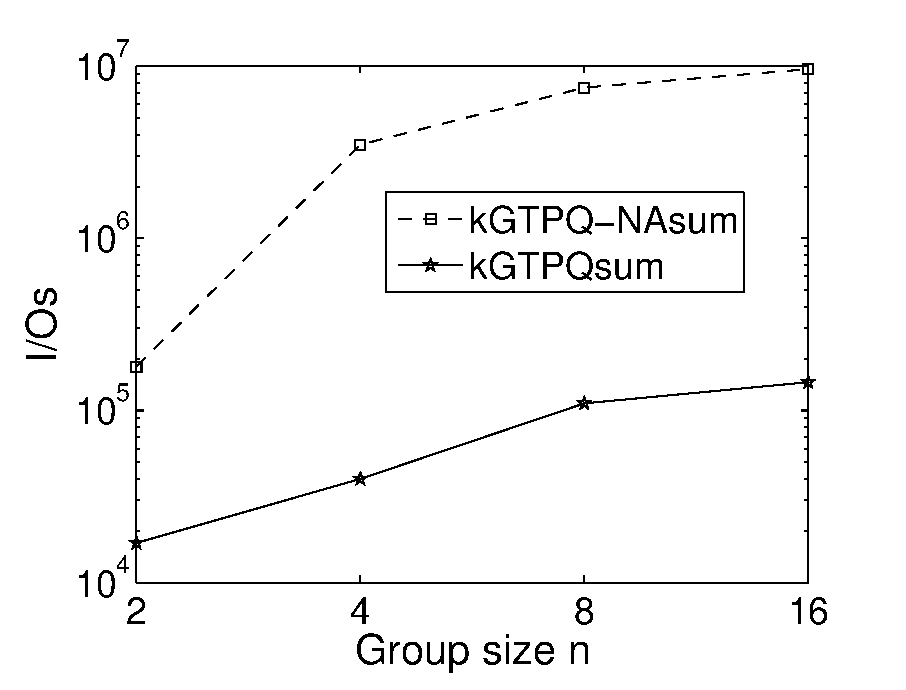
\includegraphics[]{graph/SumGIO.eps}} &
        \hspace{-5mm}
         \vspace{-2mm}
      \resizebox{70mm}{!}{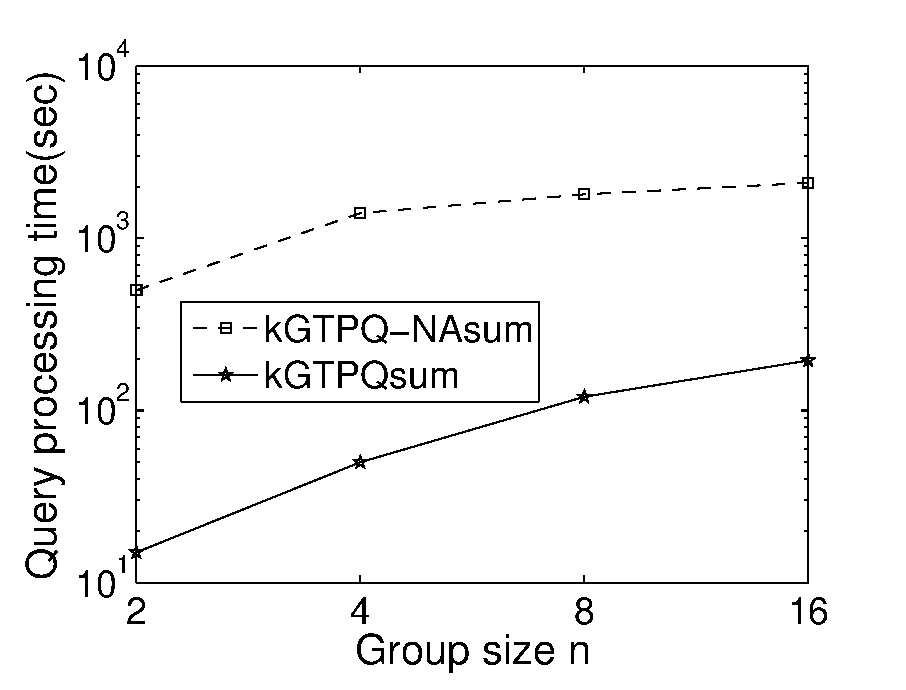
\includegraphics[]{graph/SumGTime.eps}} \\
      \scriptsize{(a) \textsc{}\hspace{0mm}} & \scriptsize{(b) \textsc{}}\\
        %\hspace{-5mm}
%        \resizebox{40mm}{!}{\includegraphics{graph/sum/vk_io.pdf}} &
%        \hspace{-5mm}
%      \resizebox{40mm}{!}{\includegraphics{graph/max/vk_io.pdf}} \\
%      \scriptsize{(c) \textsc{sum}\hspace{0mm}} & \scriptsize{(d) \textsc{max}}\\
%      \hspace{-5mm}
%      \resizebox{40mm}{!}{\includegraphics{graph/sum/vk_answer.pdf}} &
%        \hspace{-5mm}
%      \resizebox{40mm}{!}{\includegraphics{graph/max/vk_answer.pdf}} \\
%       \scriptsize{(e) \textsc{sum}\hspace{0mm}} & \scriptsize{(f) \textsc{max}}
        \end{tabular}
    \caption{Effect of group size $n$ for California data (a) I/Os and (b) query processing time}
    \label{graph:sum_g}
  \end{center}
   \vspace{-6mm}
\end{figure}

\vspace*{10pt}
\textbf{\emph{Effect of answer set $k$: }} In this set of experiments, we vary $k$ as 2, 4, 8, and 16, and compare the experimental results $kGTPQ_{sum}$ and $kGTPQ-NA_{sum}$.


From Figure ~\ref{graph:sum_k}(a) and Figure~\ref{graph:sum_k}(b), we observe that I/Os and processing time increase with the increase of $k$ for both $kGTPQ_{sum}$ and $kGTPQ-NA_{sum}$. Figures show that $kGTPQ-NA_{sum}$ takes almost one and half orders of magnitude more I/Os compared to $kGTPQ_{sum}$. We also see from Figure~\ref{graph:sum_k}(b) that the query processing time of $kGTPQ-NA_{sum}$ is on average one and
half orders of magnitude higher than that of $kGTPQ_{sum}$. The superiority of our approach over the naive approach comes from the ellipse based pruning strategies that reduces the search space significantly.

\vspace*{10pt}
\begin{figure}[htbp]
 %\vspace{-2mm}
  \begin{center}
    \begin{tabular}{cc}
         \hspace{-5mm}
      \resizebox{70mm}{!}{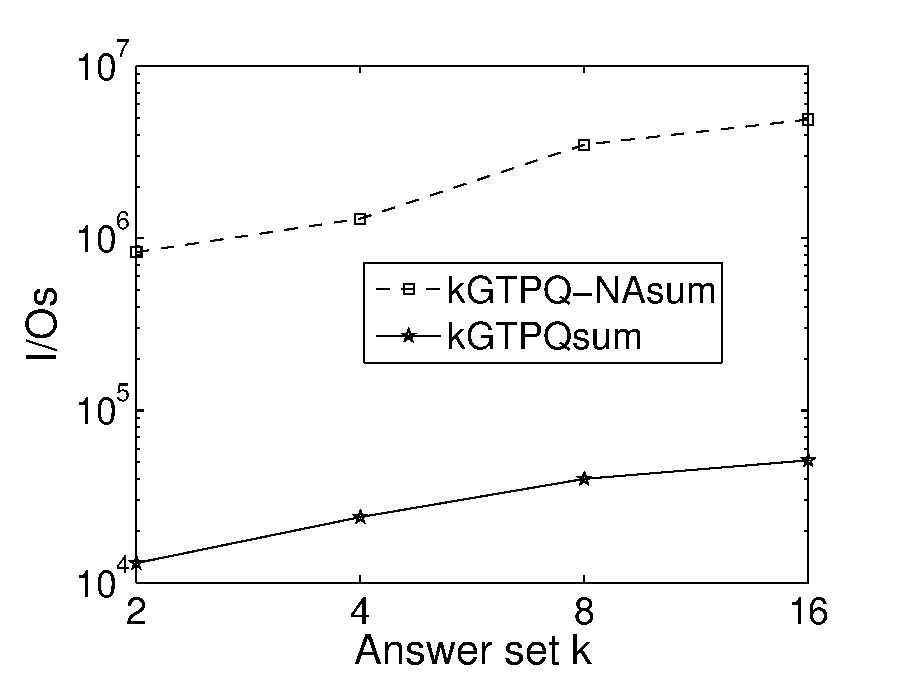
\includegraphics[]{graph/SumKIO.eps}} &
        \hspace{-5mm}
         \vspace{-2mm}
      \resizebox{70mm}{!}{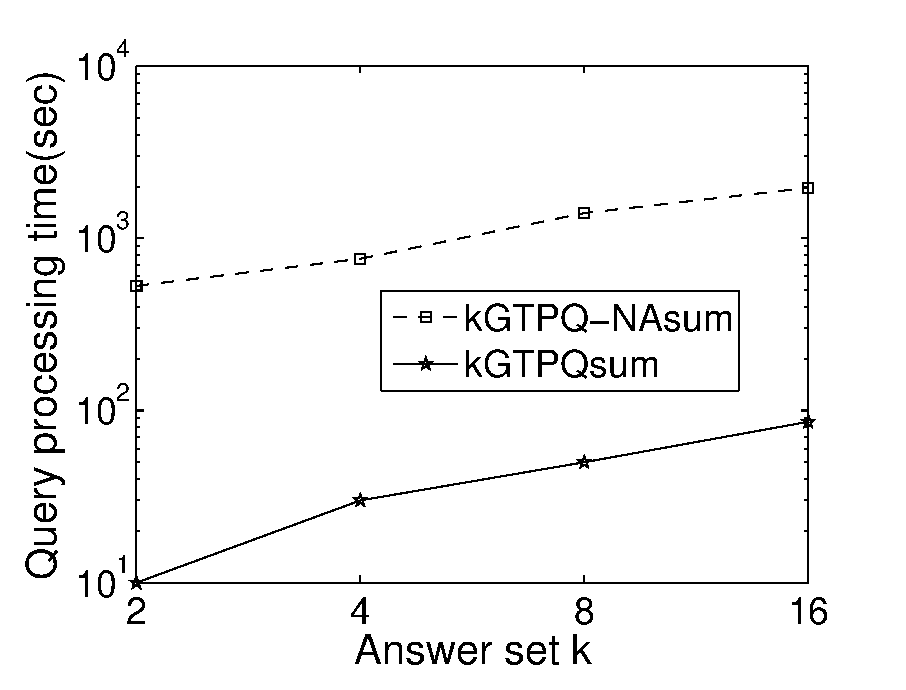
\includegraphics[]{graph/SumKTime.eps}} \\
      \scriptsize{(a) \textsc{}\hspace{0mm}} & \scriptsize{(b) \textsc{}}\\
        %\hspace{-5mm}
%        \resizebox{40mm}{!}{\includegraphics{graph/sum/vk_io.pdf}} &
%        \hspace{-5mm}
%      \resizebox{40mm}{!}{\includegraphics{graph/max/vk_io.pdf}} \\
%      \scriptsize{(c) \textsc{sum}\hspace{0mm}} & \scriptsize{(d) \textsc{max}}\\
%      \hspace{-5mm}
%      \resizebox{40mm}{!}{\includegraphics{graph/sum/vk_answer.pdf}} &
%        \hspace{-5mm}
%      \resizebox{40mm}{!}{\includegraphics{graph/max/vk_answer.pdf}} \\
%       \scriptsize{(e) \textsc{sum}\hspace{0mm}} & \scriptsize{(f) \textsc{max}}
        \end{tabular}
    \caption{Effect of answer set $k$ for California data (a) I/Os and (b) Query processing time}
    \label{graph:sum_k}
  \end{center}
   \vspace{-6mm}
\end{figure}
\vspace*{10pt}

\textbf{\emph{Effect of Query Area $M$: }}In this case, we vary the query area $M$ as 2\%, 4\%, 8\% and 16\% of the data space. Figure~\ref{graph:sum_m}(a) and ~\ref{graph:sum_m}(b) show I/Os and query processing time, required by $kGTPQ_{sum}$ and $kGTPQ-NA_{sum}$, respectively. Since we need to access more data points from $R$-trees of different data types for a larger $M$, both I/Os and processing time increase with the increase of $M$ for both approaches.


Figure~\ref{graph:sum_m}(a) shows that $kGTPQ-NA_{sum}$ requires at least one and half orders of
magnitude more I/Os than that of $kGTPQ_{sum}$. Similarly, Figure ~\ref{graph:sum_m}(b)
shows that the processing time of $kGTPQ-NA_{sum}$ is on average one order of magnitude higher
than that of $kGTPQ_{sum}$.


\vspace*{10pt}
\begin{figure}[htbp]
 %\vspace{-2mm}
  \begin{center}
    \begin{tabular}{cc}
         \hspace{-5mm}
      \resizebox{70mm}{!}{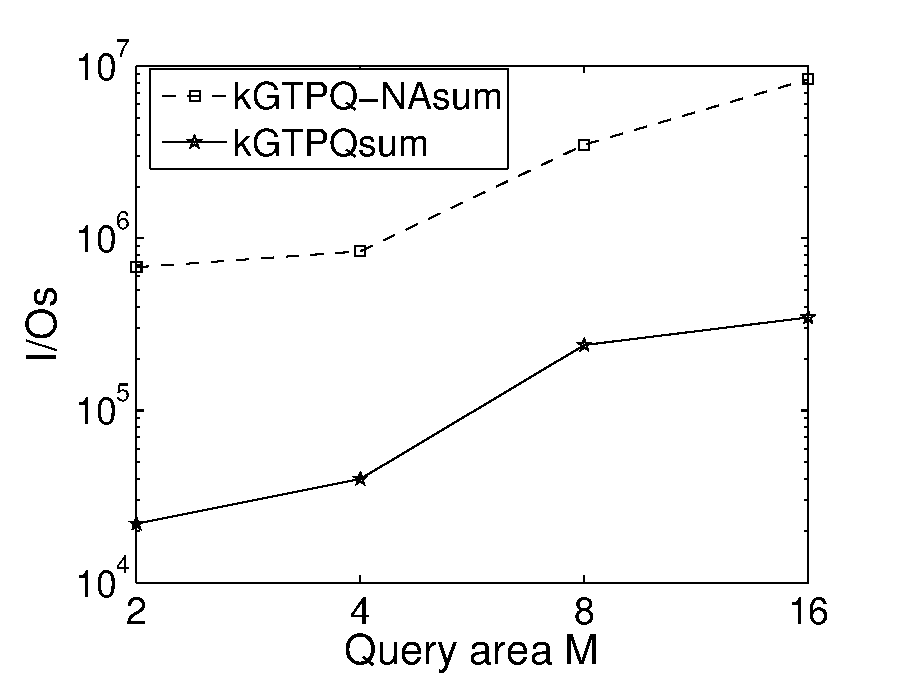
\includegraphics{graph/SumMIO.eps}} &
        \hspace{-5mm}
         \vspace{-2mm}
      \resizebox{70mm}{!}{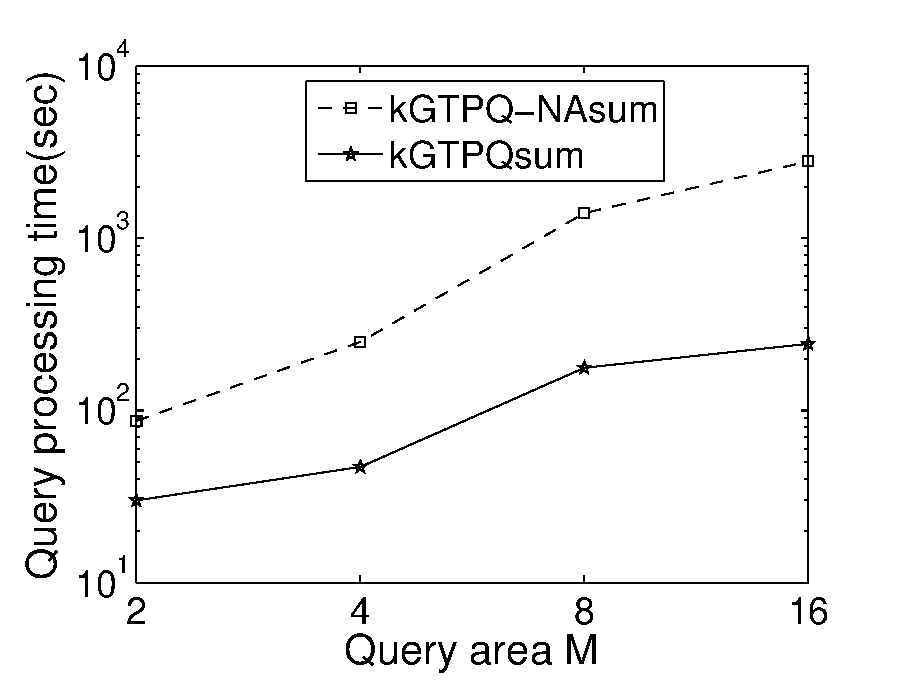
\includegraphics{graph/SumMTime.eps}} \\
      \scriptsize{(a) \textsc{}\hspace{0mm}} & \scriptsize{(b) \textsc{}}\\
        %\hspace{-5mm}
%        \resizebox{40mm}{!}{\includegraphics{graph/sum/vk_io.pdf}} &
%        \hspace{-5mm}
%      \resizebox{40mm}{!}{\includegraphics{graph/max/vk_io.pdf}} \\
%      \scriptsize{(c) \textsc{sum}\hspace{0mm}} & \scriptsize{(d) \textsc{max}}\\
%      \hspace{-5mm}
%      \resizebox{40mm}{!}{\includegraphics{graph/sum/vk_answer.pdf}} &
%        \hspace{-5mm}
%      \resizebox{40mm}{!}{\includegraphics{graph/max/vk_answer.pdf}} \\
%       \scriptsize{(e) \textsc{sum}\hspace{0mm}} & \scriptsize{(f) \textsc{max}}
        \end{tabular}
    \caption{Effect of query area $M$ for California data (a) I/Os and (b) query processing time}
    \label{graph:sum_m}
  \end{center}
   \vspace{-6mm}
\end{figure}
\vspace*{10pt}


\textbf{\emph{Effect of dataset size: }}In this set of experiments, we vary the road network size and number of POIs as stated in Table~\ref{table:exp_synthetic}. In this case, we use the first column, i.e., varying the number of nodes as 5000,
10000,15000 and 20000 to identify four synthetic datasets. Figure~\ref{graph:sum_u}(a)
and ~\ref{graph:sum_u}(b) show I/Os and processing time respectively for
different synthetic dataset sizes. As expected, the experimental results show that
$kGTPQ_{sum}$ outperforms $kGTPQ-NA_{sum}$ in a greater margin for a larger dataset size in terms
of both I/Os and query processing time. Figure~\ref{graph:sum_u}(a) shows the I/Os of $kGTPQ-NA_{sum}$ is at least on average
one and half orders of magnitude higher than that of $kGTPQ_{sum}$ and from Figure~\ref{graph:sum_u}(b), we see that the query processing time of $kGTPQ-NA_{sum}$ is on average one order of magnitude higher than that of $kGTPQ_{sum}$.


\vspace*{10pt}
\begin{figure}[htbp]
 %\vspace{-2mm}
  \begin{center}
    \begin{tabular}{cc}
         \hspace{-5mm}
      \resizebox{70mm}{!}{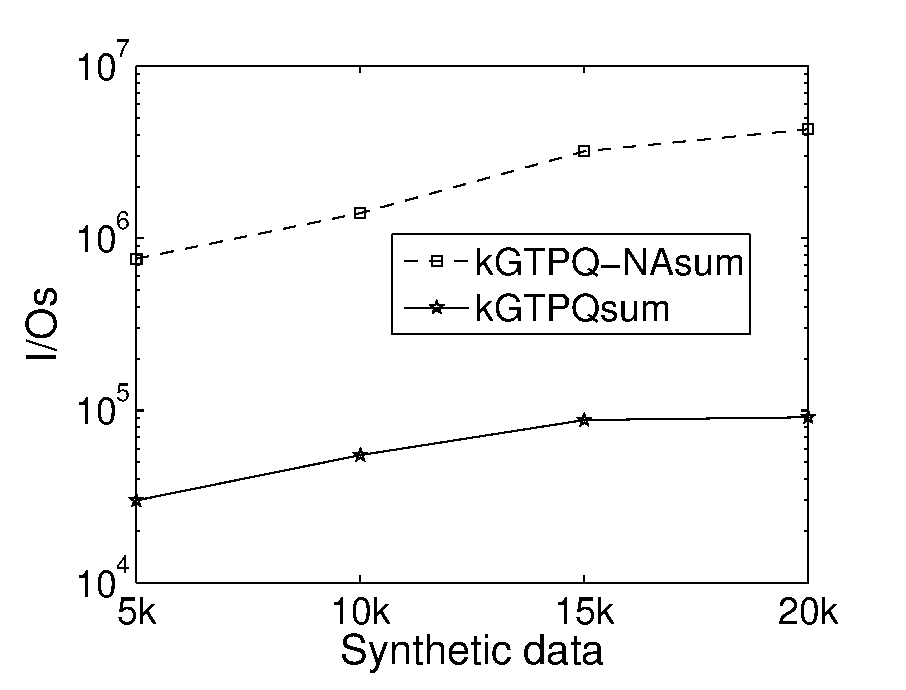
\includegraphics{graph/SumDIO.eps}} &
        \hspace{-5mm}
         \vspace{-2mm}
      \resizebox{70mm}{!}{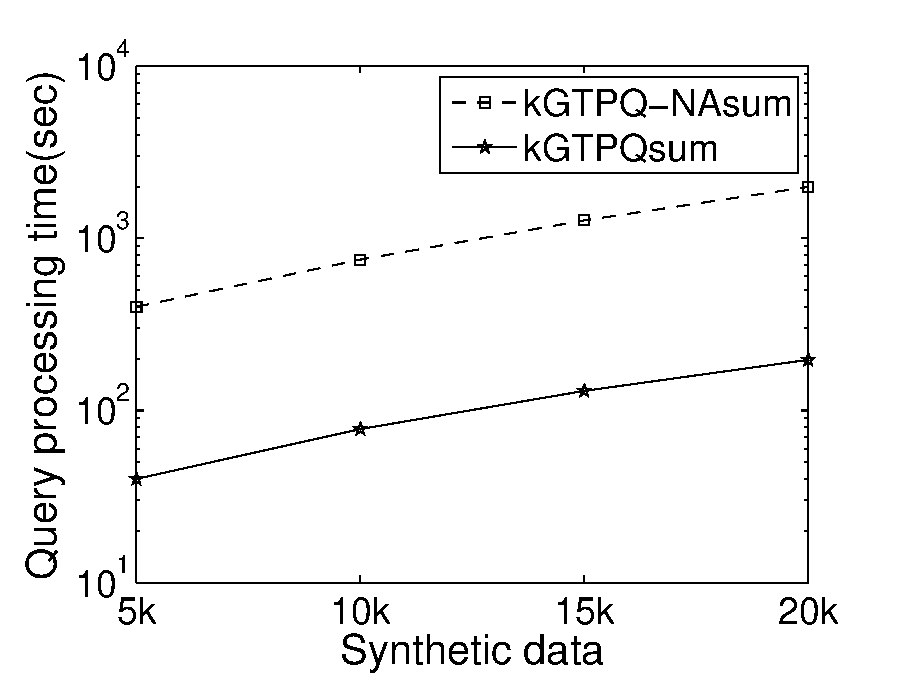
\includegraphics{graph/SumDTime.eps}} \\
      \scriptsize{(a) \textsc{}\hspace{0mm}} & \scriptsize{(b) \textsc{}}\\
        %\hspace{-5mm}
%        \resizebox{40mm}{!}{\includegraphics{graph/sum/vk_io.pdf}} &
%        \hspace{-5mm}
%      \resizebox{40mm}{!}{\includegraphics{graph/max/vk_io.pdf}} \\
%      \scriptsize{(c) \textsc{sum}\hspace{0mm}} & \scriptsize{(d) \textsc{max}}\\
%      \hspace{-5mm}
%      \resizebox{40mm}{!}{\includegraphics{graph/sum/vk_answer.pdf}} &
%        \hspace{-5mm}
%      \resizebox{40mm}{!}{\includegraphics{graph/max/vk_answer.pdf}} \\
%       \scriptsize{(e) \textsc{sum}\hspace{0mm}} & \scriptsize{(f) \textsc{max}}
        \end{tabular}
    \caption{Effect of varying dataset size (a) I/Os and (b) query processing time}
    \label{graph:sum_u}
  \end{center}
   \vspace{-6mm}
\end{figure}
\vspace*{10pt}

\subsection{Aggregate function MAX}
\label{subsec:max}
In this section, we present the experimental results for processing $k$GTP queries for aggregate function MAX. For MAX, we name our proposed approach and the naive approach as $kGTPQ_{max}$ and $kGTPQ-NA_{max}$, respectively. In the following sets of experiments, we vary group size, the answer set size, query area, and dataset size, and compare the results of our approach with the naive approach.


\textbf{\emph{Effect of group size $n$: }}Figure~\ref{graph:max_g}(a) and ~\ref{graph:max_g}(b) show I/Os and query processing times, respectively, for processing $k$GTP queries using $kGTPQ_{max}$ and $kGTPQ-NA_{max}$. For $kGTPQ-NA_{max}$, I/Os and query processing time almost remain constant with the increase of $n$. On the other hand for $kGTPQ_{max}$, I/Os and processing time slightly increase with the increase of group size from 4 to 8, and then it almost remains constant for a larger group. As expected, I/Os and query processing time of $kGTPQ_{max}$ are much less than those of $kGTPQ-NA_{max}$. Figure~\ref{graph:max_g}(a) and (b) show that I/Os and query processing time of $kGTPQ_{max}$ are on average one and half orders of magnitude smaller than those of $kGTPQ-NA_{max}$.

\vspace*{10pt}
\begin{figure}[htbp]
 %\vspace{-2mm}
  \begin{center}
    \begin{tabular}{cc}
         \hspace{-5mm}
      \resizebox{70mm}{!}{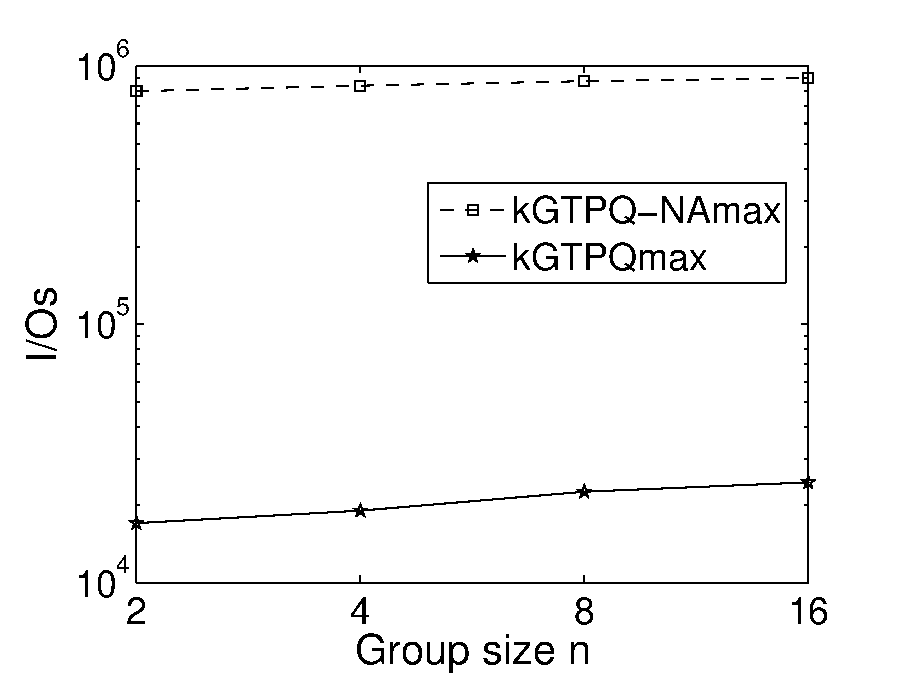
\includegraphics{graph/MaxGIO.eps}} &
        \hspace{-5mm}
         \vspace{-2mm}
      \resizebox{70mm}{!}{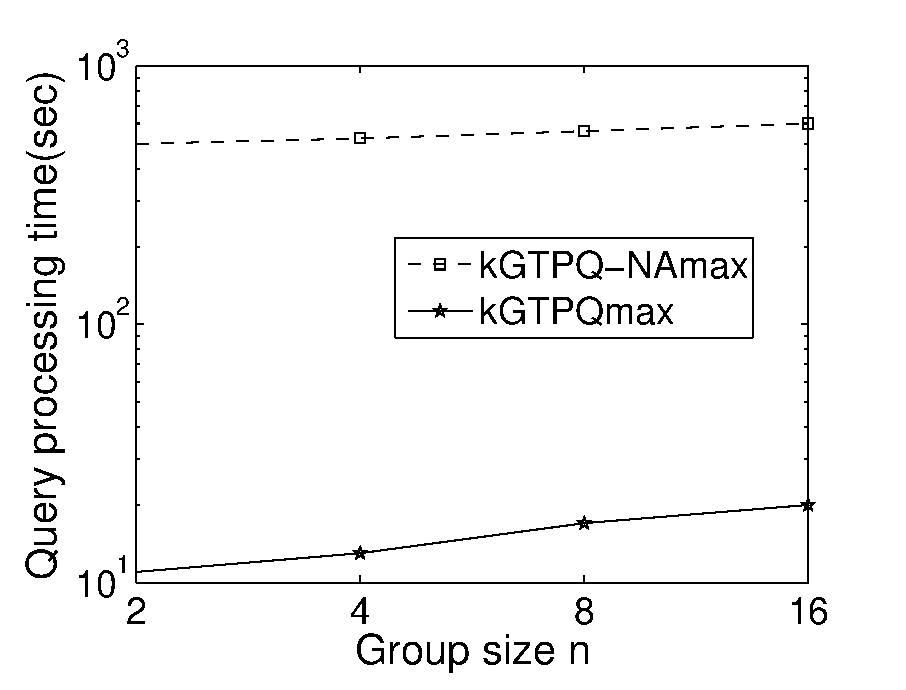
\includegraphics{graph/MaxGTime.eps}} \\
      \scriptsize{(a) \textsc{}\hspace{0mm}} & \scriptsize{(b) \textsc{}}\\
        %\hspace{-5mm}
%        \resizebox{40mm}{!}{\includegraphics{graph/sum/vk_io.pdf}} &
%        \hspace{-5mm}
%      \resizebox{40mm}{!}{\includegraphics{graph/max/vk_io.pdf}} \\
%      \scriptsize{(c) \textsc{sum}\hspace{0mm}} & \scriptsize{(d) \textsc{max}}\\
%      \hspace{-5mm}
%      \resizebox{40mm}{!}{\includegraphics{graph/sum/vk_answer.pdf}} &
%        \hspace{-5mm}
%      \resizebox{40mm}{!}{\includegraphics{graph/max/vk_answer.pdf}} \\
%       \scriptsize{(e) \textsc{sum}\hspace{0mm}} & \scriptsize{(f) \textsc{max}}
        \end{tabular}
    \caption{Effect of group size $n$ for California data (a) I/Os and (b) Query processing time)}
    \label{graph:max_g}
  \end{center}
   \vspace{-6mm}
\end{figure}
\vspace*{10pt}


\textbf{\emph{Effect of answer set $k$: }} In this set of experiments, we vary $k$ as 2, 4, 8, and 16, and compare the experimental results $kGTPQ_{max}$ and $kGTPQ-NA_{max}$.

In Figure~\ref{graph:max_k}(a), we observe that I/Os almost remain constant with the increase of $k$.
We find that $kGTPQ-NA_{max}$ takes almost two orders of magnitude
more I/Os compare to $kGTPQ_{max}$. Figure~\ref{graph:max_k}(b) shows that the query processing time of $kGTPQ-NA_{max}$ is at least one and half order of magnitude higher than that of $kGTPQ_{max}$ because it facilitates ellipse based pruning to reduce the search space significantly.



\vspace*{10pt}
\begin{figure}[htbp]
 %\vspace{-2mm}
  \begin{center}
    \begin{tabular}{cc}
         \hspace{-5mm}
      \resizebox{70mm}{!}{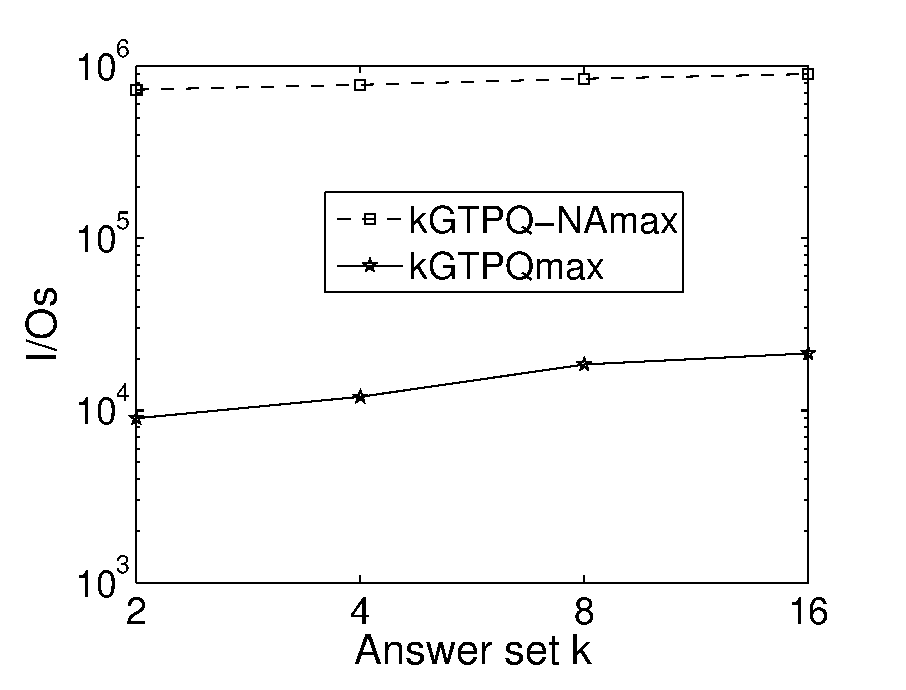
\includegraphics[width=\textwidth]{graph/MaxKIO.eps}} &
        \hspace{-5mm}
         \vspace{-2mm}
      \resizebox{70mm}{!}{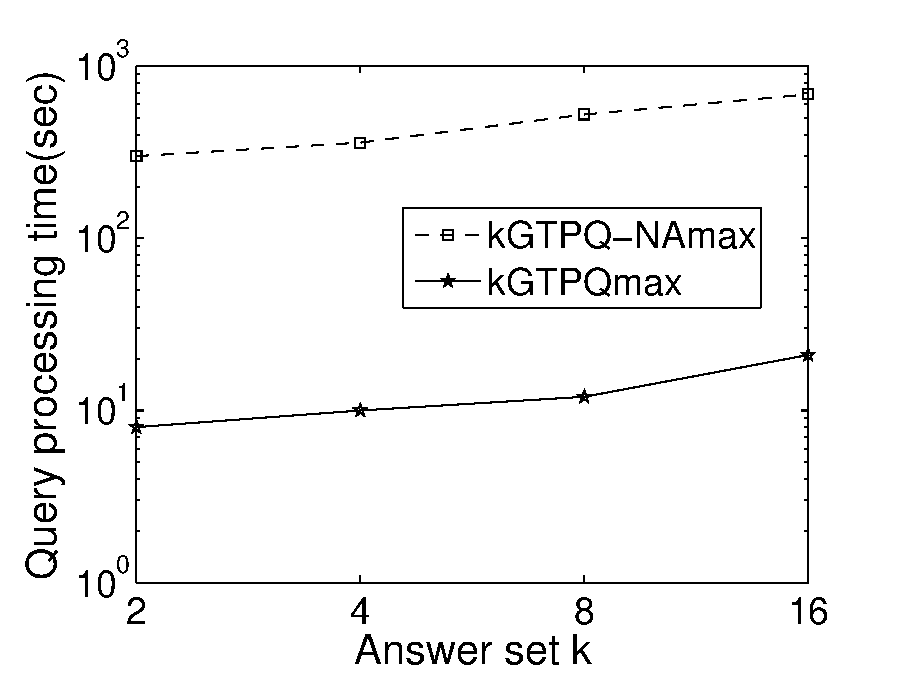
\includegraphics{graph/MaxKTime.eps}} \\
      \scriptsize{(a) \textsc{}\hspace{0mm}} & \scriptsize{(b) \textsc{}}\\
        %\hspace{-5mm}
%        \resizebox{40mm}{!}{\includegraphics{graph/sum/vk_io.pdf}} &
%        \hspace{-5mm}
%      \resizebox{40mm}{!}{\includegraphics{graph/max/vk_io.pdf}} \\
%      \scriptsize{(c) \textsc{sum}\hspace{0mm}} & \scriptsize{(d) \textsc{max}}\\
%      \hspace{-5mm}
%      \resizebox{40mm}{!}{\includegraphics{graph/sum/vk_answer.pdf}} &
%        \hspace{-5mm}
%      \resizebox{40mm}{!}{\includegraphics{graph/max/vk_answer.pdf}} \\
%       \scriptsize{(e) \textsc{sum}\hspace{0mm}} & \scriptsize{(f) \textsc{max}}
        \end{tabular}
    \caption{Effect of answer set $k$ for California data (a) I/Os and (b) Query processing time}
    \label{graph:max_k}
  \end{center}
   \vspace{-6mm}
\end{figure}
\vspace*{10pt}


\textbf{\emph{Effect of query area $M$: }}In this set of experiments, we vary the query area $M$ as 2\%,4\%,8\%,16\% of entire data space. Figure~\ref{graph:max_m}(a) and ~\ref{graph:max_m}(b) show that I/Os
and processing time, respectively, for $kGTPQ_{max}$ and $kGTPQ-NA_{max}$. We observe that I/Os
and query processing time increase with the increase of $M$ for both algorithms
as for a larger $M$ both approaches need to access more data points from R-trees than those of a smaller
$M$.

Figure~\ref{graph:max_m}(a) shows that $kGTPQ-NA_{max}$ requires at least two orders of
magnitude more I/Os than that of $kGTPQ_{max}$. Similarly, Figure ~\ref{graph:max_m}(b)
shows that the query processing time of $kGTPQ-NA_{max}$ is on average one and half orders of magnitude higher
than that of $kGTPQ_{max}$.

\vspace*{10pt}
\begin{figure}[htbp]
 %\vspace{-2mm}
  \begin{center}
    \begin{tabular}{cc}
         \hspace{-5mm}
      \resizebox{70mm}{!}{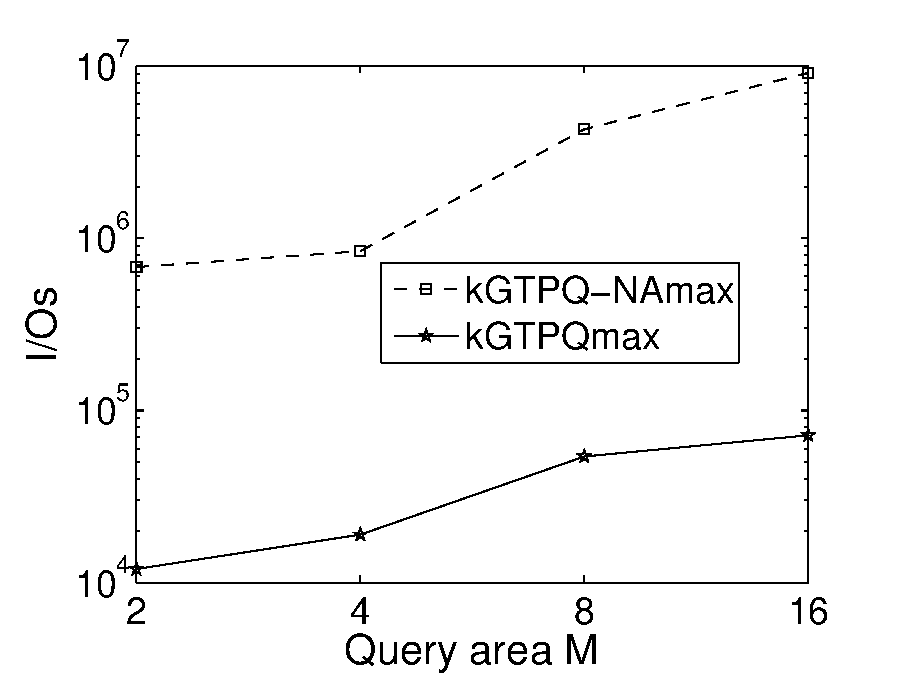
\includegraphics{graph/MaxMIO.eps}} &
        \hspace{-5mm}
         \vspace{-2mm}
      \resizebox{70mm}{!}{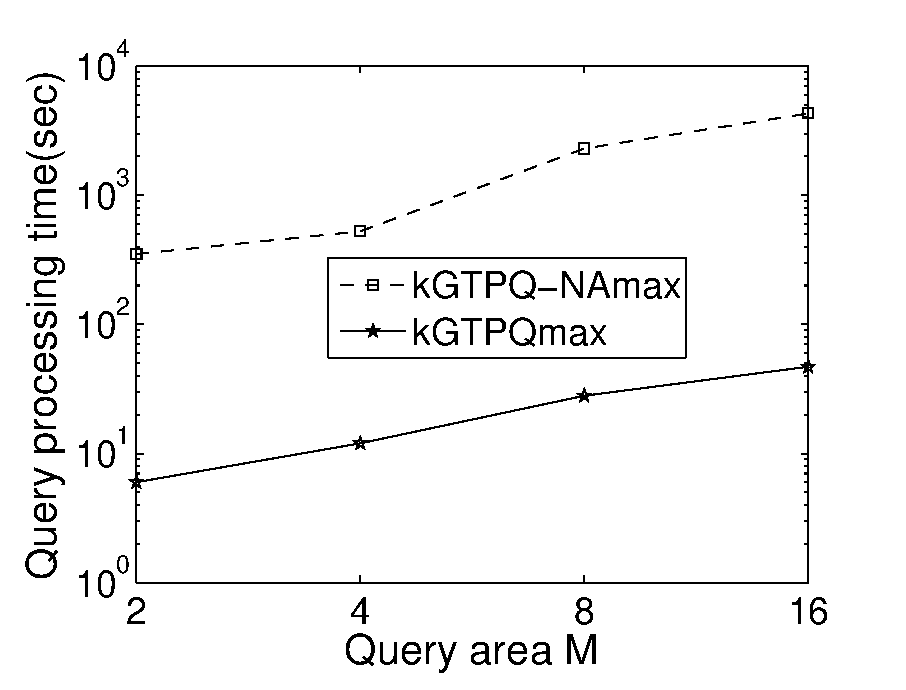
\includegraphics{graph/MaxMTime.eps}} \\
      \scriptsize{(a) \textsc{}\hspace{0mm}} & \scriptsize{(b) \textsc{}}\\
        %\hspace{-5mm}
%        \resizebox{40mm}{!}{\includegraphics{graph/sum/vk_io.pdf}} &
%        \hspace{-5mm}
%      \resizebox{40mm}{!}{\includegraphics{graph/max/vk_io.pdf}} \\
%      \scriptsize{(c) \textsc{sum}\hspace{0mm}} & \scriptsize{(d) \textsc{max}}\\
%      \hspace{-5mm}
%      \resizebox{40mm}{!}{\includegraphics{graph/sum/vk_answer.pdf}} &
%        \hspace{-5mm}
%      \resizebox{40mm}{!}{\includegraphics{graph/max/vk_answer.pdf}} \\
%       \scriptsize{(e) \textsc{sum}\hspace{0mm}} & \scriptsize{(f) \textsc{max}}
        \end{tabular}
    \caption{Effect of Query Area $M$ for California data (a) I/Os and (b) Query processing time}
    \label{graph:max_m}
  \end{center}
   \vspace{-6mm}
\end{figure}
\vspace*{10pt}


\textbf{\emph{Effect of dataset sizes: }} Similar to SUM, In this set of experiments, we vary the road network size and number of POIs as stated in Table~\ref{table:exp_synthetic}.

Figure~\ref{graph:max_u}(a) and~\ref{graph:max_u}(b) show I/Os and processing time, respectively, for
different dataset sizes. The experimental results show that
$kGTPQ_{max}$ outperforms $kGTPQ-NA_{max}$ for all dataset sizes in terms
of both I/Os and query processing time.

Figure ~\ref{graph:max_m}(a)
shows that I/Os of $kGTPQ-NA_{max}$ is on average one and half orders of magnitude higher
than that of $kGTPQ_{max}$.
Figure ~\ref{graph:max_m}(b)
shows that query processing time of $kGTPQ-NA_{max}$ is on average one and half orders of magnitude higher
than that of $kGTPQ_{max}$.

\vspace*{10pt}
\begin{figure}[htbp]
 %\vspace{-2mm}
  \begin{center}
    \begin{tabular}{cc}
         \hspace{-5mm}
      \resizebox{70mm}{!}{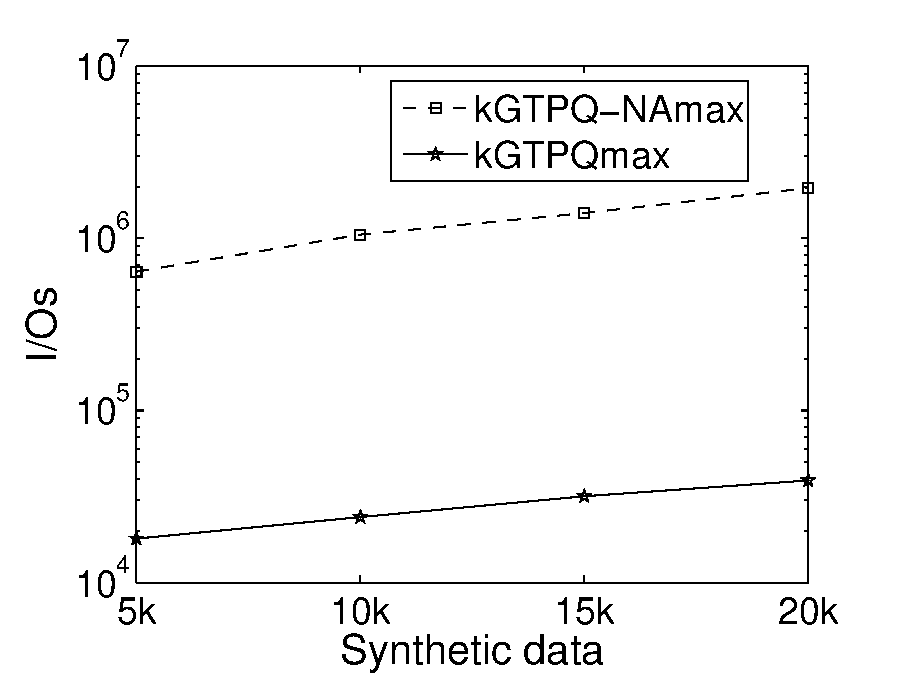
\includegraphics{graph/MaxDIO.eps}} &
        \hspace{-5mm}
         \vspace{-2mm}
      \resizebox{70mm}{!}{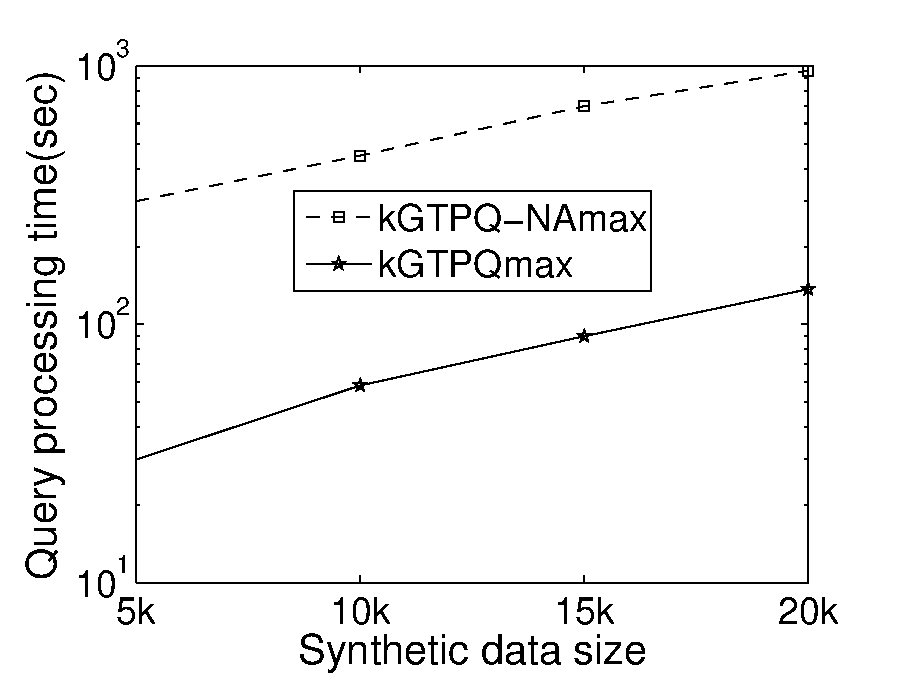
\includegraphics{graph/MaxDTime.eps}} \\
      \scriptsize{(a) \textsc{}\hspace{0mm}} & \scriptsize{(b) \textsc{}}\\
        %\hspace{-5mm}
%        \resizebox{40mm}{!}{\includegraphics{graph/sum/vk_io.pdf}} &
%        \hspace{-5mm}
%      \resizebox{40mm}{!}{\includegraphics{graph/max/vk_io.pdf}} \\
%      \scriptsize{(c) \textsc{sum}\hspace{0mm}} & \scriptsize{(d) \textsc{max}}\\
%      \hspace{-5mm}
%      \resizebox{40mm}{!}{\includegraphics{graph/sum/vk_answer.pdf}} &
%        \hspace{-5mm}
%      \resizebox{40mm}{!}{\includegraphics{graph/max/vk_answer.pdf}} \\
%       \scriptsize{(e) \textsc{sum}\hspace{0mm}} & \scriptsize{(f) \textsc{max}}
        \end{tabular}
    \caption{Effect of synthetic data set (a) I/Os and (b) Query processing time}
    \label{graph:max_u}
  \end{center}
   \vspace{-6mm}
\end{figure}
\vspace*{10pt}



\begin{table}[htbp]
  \centering
\begin{tabular}{|c|c|c|}
  \hline
  % after \\: \hline or \cline{col1-col2} \cline{col3-col4} ...
  Parameter& $kGTPQ_{sum}$ & $kGTPQ_{max}$\\
  \hline
  Group size $n$ & 78225 & 20737 \\
  \hline
  Query area $M$& 162250 & 39198\\
  \hline
  $k$ & 32086 & 15240\\
  \hline
  Synthetic data set & 66080 & 28251 \\
  \hline
\end{tabular}
\caption{Average I/Os for $kGTPQ_{sum}$ and $kGTPQ_{max}$ for different parameters} \label{table:IO_Overhead} \vspace{-2mm}
\end{table}
\vspace*{10pt}


\begin{table}[htbp]
  \centering
\begin{tabular}{|c|c|c|}
  \hline
  % after \\: \hline or \cline{col1-col2} \cline{col3-col4} ...
  Parameter& $kGTPQ_{sum}$ & $kGTPQ_{max}$\\
  \hline
  Group size $n$ & 95s & 15.25s \\
  \hline
  Query area $M$& 102.13s & 23.29s\\
  \hline
  $k$ & 44.03s & 12.76s\\
  \hline
  Synthetic data set & 111.21s & 78.37s \\
  \hline
\end{tabular}
\caption{Average query processing time for $kGTPQ_{sum}$ and $kGTPQ_{max}$ for different parameters} \label{table:Time} \vspace{-2mm}
\end{table}

\vspace*{10pt}


\subsection{Comparison between SUM and MAX}
\label{subsec:cmp}

In this section, we compare I/Os and processing time of $k$GTPQ queries for aggregate functions SUM and MAX. Tables 3 and 4 summarize I/Os and query processing time, respective, by varying different parameters.

We observe that $kGTPQ_{sum}$ requires much higher I/Os and processing time than $kGTPQ_{max}$. The underlying reason is as follows. $kGTPQ_{max}$ considers the maximum distance of any user while $kGTPQ_{sum}$ considers the total distance of all users. As the total distance of all users is larger than the maximum distance of any user, the area of the pruning ellipse for $kGTPQ_{sum}$ is much larger than that of $kGTPQ_{max}$. Hence, $kGTPQ_{sum}$ accesses higher number of R-tree nodes than $kGTPQ_{max}$.

We have also done the experiments for $m=2$. We omit the experimental results for $m=2$ as the behavior is similar to what we have described in previous sections for $m=3$. However, the processing time and I/Os for $m=3$ are higher than that of $m=2$, which is expected. Since in real scenarios, the number of data point categories is typically limited to 2 or 3, the trend of increasing performance overhead with an increase of $m$ would not effect the applicability of our algorithms.



\endinput 